\capitulo{3}{Conceptos teóricos}

Es fundamental pensar en el usuario final de una página web en el desarrollo de la misma, ya que una interfaz intuitiva y sencilla permitirá una buena interacción entre el usuario y esta. Es por ello que se ha realizado un Diseño Centrado en el Usuario.
\section{Diseño web centrado en el usuario}
El diseño esta basado en que el usuario pueda conseguir sus objetivos, como encontrar información comunicarse y aprender.

Para tratar de conseguir los objetivos del usuario, es necesario conocer estos desde el principio del desarrollo. Por ello es necesario conocer el usuario, el uso que se va a dar de la aplicación o que es lo que necesita.

Centrar el diseño en los usuario lleva a investigar la reacción ante el diseño, conocer la experiencia de uso e innovar, siempre teniendo en cuanta mejorar la experiencia del usuario.

El Diseño Web Centrado en el Usuario se divide en varias fases. Como podemos observar en la Figura \ref{fig:DisCenUsu} algunas de las fases son iterativas.
\begin{figure}
\centering
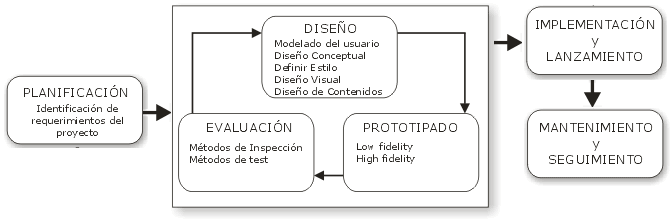
\includegraphics[width=.9\textwidth]{img/diseno_centrado_usuario}
\caption[Fases del Diseño Centrado en el Usuario.]{Imagen extraida de~\url{http://asanzdiego.github.io/curso-interfaces-web-2014/01-usabilidad/slides/img/disenio-centrado-usuario.png}}
\label{fig:DisCenUsu}
\end{figure}
\subsection{Planificación}
En necesaria una correcta planificación donde se identifiquen los objetivos, necesidades y requerimientos. En esta fase va a dividirse en etapas más pequeñas:

\subsubsection{Modelado del usuario}
Lo primero es tener en cuenta aquellas clases o perfiles de usuarios, que vamos a necesitar. Tendremos en cuenta la información a la que necesitan acceder, las condiciones de acceso y su experiencia y conocimientos. Así se tener  en cuenta para quien diseñar y lo que el usuario puede esperar encontrar.

\subsubsection{Diseño conceptual}
Se va a elaborar la estructura del sitio web, con estructura nos referimos a las conexiones y relaciones entre páginas y la posible navegación entre estas mismas. La arquitectura puede ser descendente donde nos desplazamos de lo general a las partes y ascendente, donde el desempeño global se logra con bloques mínimos de información.

\subsubsection{Diseño visual}
La facilidad con la que encontrar información, tiene que ver con la distribución que se hace de esta. La zona superior, por ejemplo, tiene una mayor jerarquía visual que las inferiores y es por ello que encontramos información más valiosa. Para variar la jerarquía de la información se utiliza diferente tamaño de letra o diferente fuente.

Lo importante es mantener una coherencia de diseño en todas las páginas. Un elemento que nos puede ayudar a lograr esto, son las páginas maestras.

\subsubsection{Diseño de contenidos}
El texto que nos encontremos debe tener un diseño y es que no puede ser caótico, de manera que encontrar la información resulte una quimera. Algunas características que debe tener son: tono cercano y familiar, conciso y preciso y que todo párrafo resuma una idea.
Todo ello facilita enormemente que el usuario pueda localizar más fácilmente la información que desea.

\subsection{Prototipado}
Es necesario hacer prototipos de las interfaz del sitio que no tienen por que ser iguales al modelo final, pero nos servirán para evaluar la usabilidad del  sitio web sin tener que implementarla.

En un primer momento se puede realizar un prototipo en papel, donde veamos de una manera sencilla la distribución de la web. También existe software capaz de ayudarnos a realizar prototipos con este software incluso podemos interactuar con las diferentes páginas.

\subsection{Evaluación de la usabilidad}
Aunque hay diversas maneras de evaluar la usabilidad de un sitio web nos vamos a centrar en el test con usuarios ya que es el que se ha llevado a cabo.

Se va a realizar un análisis con un grupo de usuarios utilizando la web y se va apuntando aquellos problemas con los que se van encontrando. Los mismos usuarios muchas veces proporcionan algunas ideas que nos pueden permitir solventar algunos problemas. Es importante que los usuarios con los que se lleva a cabo la evaluación de usabilidad, tengan el mismo perfil o similar al del usuario final. Por ejemplo si elaboramos un sitio web para un tipo de usuario más experto, es normal que un usuario básico se encuentre con una infinidad de problemas, que el usuario experto no.

\subsection{Implementación y lanzamiento}
Es muy recomendable elaborar un sitio web con los estándares, ya que esto nos asegura que en el futuro haya una compatibilidad del sitio además de permitir un futuro crecimiento del mismo.
También es importante el uso de hojas de diseño y bases de datos, ya que permite que si en un futuro hay que readaptar las necesidades, resulte más sencillo.

Una vez lanzado el sitio web los primeros meses son muy importantes, los usuarios son primerizos y deben encontrar una facilidad de uso, tambien podemos hacer pequeños tutoriales que enseñen a utilizar el sitio web.

Para mantener una correcta promoción del sitio es necesario incluir la empresa en banners, en buscadores o publicitarse a través del correo electrónico.

\subsection{Mantenimiento y seguimiento}
Según va pasando el tiempo es importante realizar un seguimiento de los usuarios que se conectan periódicamente a la web, ya que es este el volumen importante de usuarios. Hay que analizar por qué aquellos usuarios que se conectan por primera vez no lo vuelven a hacer. Una forma de hacerlo es generar un apartado de opinión de usuarios, donde estos nos expongan su opinión del sitio web para analizarlo más adelante.

Otras preguntas que debemos realizarnos son: ¿quién lo utiliza?, ¿cuándo lo utiliza?, ¿desde dónde lo utiliza?, ¿qué utiliza?
Es muy importante tener una respuesta a estas preguntas, ya que nos puede permitir adaptarnos a los usuarios y de esta manera afianzarnos a ellos.

\section{Scraping}
Técnica utilizada para simular  la navegación de un humano en Internet con el fin de extraer información del sitio web. Los datos pueden ser almacenados y analizados en una base de datos cent no expandimos ral o en otros lugares de almacenamiento.  Son diversas las técnicas que se pueden utilizar, en concreto se ha empleado el protocolo HTTP, mediante la observación de la estructura de la página vamos viendo como recorrerla y cuál es el sitio en el que encontramos los datos que queremos, una vez ahí los extraemos.\cite{_web_2016}

\section{Machine Learning}
En español denominado como aprendizaje automático, es aquel proceso que le da a las computadoras la habilidad de aprender sin ser explícitamente programadas. Hay una segunda definición mucho más clara:
\begin{quote}
Se dice que un programa de computación aprende de la experiencia E con respecto a una tarea T y alguna medida de rendimiento P, si el rendimiento en T, medido por P, mejora con la experiencia E.
\end{quote}
El Machine Learning se divide en dos áreas principales, el aprendizaje supervisado y el no supervisado, mientras que el primero requiere una etiqueta a predecir, en el segundo no se sabe.\cite{_machine_learning_2014}

En esta figura \ref{fig:EjMachLear} podemos ver un ejemplo sencillo del aprendizaje automático.

\begin{figure}
\centering
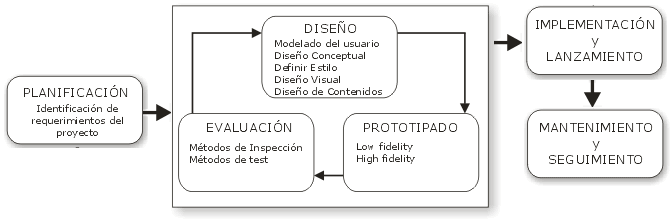
\includegraphics[width=.9\textwidth]{img/diseno_centrado_usuario}
\caption[Sencillo ejemplo de Machine Learning]{Imagen proportionada por Álvar Arnaiz}}
\label{fig:EjMachLear}
\end{figure}

\section{Minería de datos} Es el proceso por el cual es posible detectar información tratable de conjuntos de datos, para después transformarla en una estructura comprensible y poder así utilizarla más tarde.
Tiende a confundirse con el Machine Learning, pero su principal diferencia es que mientras este último se usa para reproducir patrones conocidos y hacer predicciones basadas en patrones, la minería de datos descubre patrones desconocidos.

\section{Neuronas artificiales}
Similares a la idea de neuronas biológicas, forman parte de redes neuronales artificiales. Reciben una serie de entradas y dan una salida, la cual se ve condicionada por tres funciones: función de propagación, función de activación y función de transferencia.

\section{Redes neuronales artificiales}
Imitan el funcionamiento de las redes neuronales biológicas, donde un conjunto de neuronas artificiales trabajan unidas, a fin de resolver problemas relacionados con el reconocimiento de formas o con la predicción. Se parte de un conjunto de datos de entrada significativo para conseguir que la red aprenda las propiedades deseadas\cite{.

\section{Aprendizaje Supervisado}
Se dispone de un conjunto de ejemplos de el cual se conoce la respuesta, por lo que el objetivo es marcar una regla o correspondencia de manera que sea posible aproximar la respuesta para todos los objetos que se presenten. La salida de la función puede ser un valor numérico o una clase~\cite{contributors_phpmyadmin_????}.
El uso más extendido del aprendizaje supervisado consiste en hacer predicciones a futuro basadas en comportamientos o características ya vistas en los datos que se contienen\cite{_conceptos_2014}

\section{Backpropagation}
También denominada propagación hacia atrás de errores, es un tipo de algoritmo con aprendizaje supervisado utilizado para el entrenamiento de las redes neuronales artificiales. Una vez aplicado un patrón, este se propaga a través del resto de capas hasta generar una salida, la cual se compara con la salida establecida como objetivo ya que se trata de aprendizaje supervisado. Se obtiene un error que se propaga hacia atrás cambiando los pesos, acercando así el algoritmo a un mejor resultado.
A medida que se entrena la red neuronal, las capas intermedias aprenden a organizarse para así reconocer diferentes características del espacio de entrada~\cite{mazur_step_2015}.

\section{Preprocesamiento}
El ruido y las anomalías de las bases de datos reales suelen conducir a la extracción de patrones y reglas poco útiles. La finalidad del preprocesamiento es la creación de información homogénea. En el proyecto se ha llevado a cabo la normalización

\section{Demonios}
También llamados servicios, son un tipo especial de procesos que se ejecutan en segundo plano.
El sistema los inicia en el arranque, ejecutándose en este caso una tarea planificada y comprobando si la fecha del sistema coincide con las fechas de la jornada. Para la ejecución del demonio se emplea un gestor de servicios, llamado cron. El demonio también es posible ejecutarlo a mano ya que es posible que en un momento determinado no se encuentre el servidor iniciado y no haya sido posible la ejecución del demonio\cite{torres_servicios_2013}.